%%%% Better Poster latex template example v1.0 (2019/04/04)
%%%% GNU General Public License v3.0
%%%% Rafael Bailo
%%%% https://github.com/rafaelbailo/betterposter-latex-template
%%%%
%%%% Original design from Mike Morrison
%%%% https://twitter.com/mikemorrison

\documentclass[a0paper,fleqn]{betterposter}
\usepackage{float}
%%%% Uncomment the following commands to customise the format

%% Setting the width of columns
% Left column
%\setlength{\leftbarwidth}{0.25\paperwidth}
% Right column
%\setlength{\rightbarwidth}{0.25\paperwidth}

%% Setting the column margins
% Horizontal margin
%\setlength{\columnmarginvertical}{0.05\paperheight}
% Vertical margin
%\setlength{\columnmarginhorizontal}{0.05\paperheight}
% Horizontal margin for the main column
%\setlength{\maincolumnmarginvertical}{0.15\paperheight}
% Vertical margin for the main column
%\setlength{\maincolumnmarginhorizontal}{0.15\paperheight}

%% Changing font sizes
% Text font
%\renewcommand{\fontsizestandard}{\fontsize{28}{35} \selectfont}
% Main column font
%\renewcommand{\fontsizemain}{\fontsize{28}{35} \selectfont}
% Title font
%\renewcommand{\fontsizetitle}{\fontsize{28}{35} \selectfont}
% Author font
%\renewcommand{\fontsizeauthor}{\fontsize{28}{35} \selectfont}
% Section font
%\renewcommand{\fontsizesection}{\fontsize{28}{35} \selectfont}

%% Changing font sizes for a specific text segment
% Place the text inside brackets:
% {\fontsize{28}{35} \selectfont Your text goes here}

%% Changing colours
% Background of side columns
%\renewcommand{\columnbackgroundcolor}{black}
% Font of side columns
%\renewcommand{\columnfontcolor}{gray}
% Background of main column
%\renewcommand{\maincolumnbackgroundcolor}{empirical}
%\renewcommand{\maincolumnbackgroundcolor}{theory}
%\renewcommand{\maincolumnbackgroundcolor}{methods}
%\renewcommand{\maincolumnbackgroundcolor}{intervention}
% Font of main column
%\renewcommand{\maincolumnfontcolor}{gray}

\begin{document}
\betterposter{
%%%%%%%% MAIN COLUMN

\maincolumn{
%%%% Main space

\textbf{Function-Fiasco}, an automatic detection tool, uncovers pseudo-tested methods in Python based systems.
}{
%%%% Bottom space

%% QR code
\qrcode{img/qrcode}{img/smartphoneWhite}{
\textbf{Take a picture} to
\\download the full paper
}
% Smartphone icon
% Author: Freepik
% Retrieved from: https://www.flaticon.com/free-icon/smartphone_65680

%% Compact QR code (comment the previous command and uncomment this one to switch)
%\compactqrcode{img/qrcode}{
%\textbf{Take a picture} to
%\\download the full paper
%}

}

}{
%%%%%%%% LEFT COLUMN

\title{Automatic Detection of Pseudo-tested Methods using Python and Pytest}
\author{Nicholas Tocci}
\author{Gregory Kapfhammer}

\section{Introduction}
Here is an itemised list:
\begin{itemize}
\item The first item.
\item The second item.
\item The third item.
\end{itemize}

\section{A Diagram}
Here is a diagram:
\begin{center}
% Linear regression
% Author: Henri Menke
% Retrieved from: http://www.texample.net/tikz/examples/linear-regression/
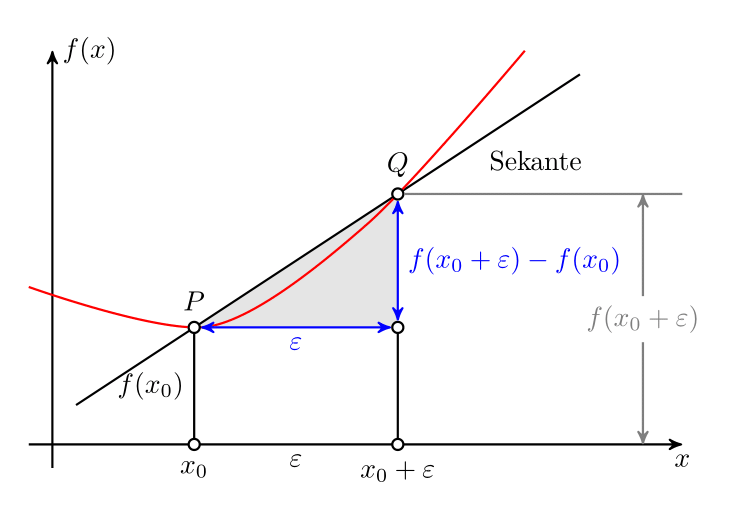
\includegraphics[width=\textwidth]{img/tikzexample1}
\end{center}

\section{Fundamental Theorem\\of Calculus}
If $f$ is continuous on the closed interval $[a,b]$ and $F$ is the indefinite integral of $f$ on $[a,b]$, then
\begin{equation}
\int_a^b f(x)\,\mathrm{d}x = F(b)-F(a).
\end{equation}


%% This fills the space between the content and the logo
\vfill

%% Institution logo
\center{

\includegraphics[scale=.95]{img/CollegeLogo}\\
}
}{
%%%%%%%% RIGHT COLUMN
\section{Results}
\begin{table}[H]
\centering

\huge

% \begingroup\small

% \begin{tabular}{rlrrrrrrrrr}
%   \hline

%  & Program & Coverage & Function Cov & NUMM & NUMTM & Fiascoed & Pseudo & NUMTTM & UC & Change \\
%   \hline

%   1 & Hashids-Python & 0.97 & 0.94 &  16 &  15 &  10 &  8 &   7 & 0.44 & 0.50 \\

%   2 & Bleach & 0.48 & 0.41 & 368 & 152 &   8 &   2 & 150 & 0.41 & 0.00 \\

%   3 & Pycco & 0.77 & 0.86 &  22 &  19 &   6 &   5 &  14 & 0.64 & 0.22 \\

%   4 & Howdoi & 0.78 & 0.95 &  20 &  19 &   2 &   0 &  19 & 0.95 & 0.00 \\

%   5 & Flashtext & 0.81 & 0.33 &  42 &  14 &   7 &   4 &  10 & 0.24 & 0.09 \\

%   6 & Honcho & 0.85 & 0.69 &  58 &  40 &   7 &   5 &  35 & 0.60 & 0.09 \\

%   7 & Maya & 0.90 & 0.50 &  88 &  44 &  13 &   3 &  41 & 0.47 & 0.03 \\

%   8 & Gator & 0.99 & 0.86 &  92 &  79 &  54 &  30 &  49 & 0.53 & 0.33 \\

%   9 & Hatch & 1.00 & 0.56 & 134 &  75 &  14 &   6 &  69 & 0.51 & 0.05 \\

%   10 & Nikola & 0.67 & 0.44 & 732 & 319 &  16 &   9 & 310 & 0.42 & 0.02 \\

%    \hline

% \end{tabular}

\begin{tabular}{r|cccc}
  % \hline

  % OLD:
  %  & Program & Coverage & Function Cov & NUMM & NUMTM & Fiascoed & Pseudo & NUMTTM & UC & Change \\
  %  \hline

  Program & Coverage & Total & Modified & Pseudo-Tested \\
  \hline

  % OLD:
  % 1 & Hashids-Python & 0.97 & 0.94 &  16 &  15 &  10 &  8 &   7 & 0.44 & 0.50 \\
  %
  Hashids-Python & 97\% & 16 & 10 & 8 \\

  % 2 & Bleach & 0.48 & 0.41 & 368 & 152 &   8 &   2 & 150 & 0.41 & 0.00 \\

  % 3 & Pycco & 0.77 & 0.86 &  22 &  19 &   6 &   5 &  14 & 0.64 & 0.22 \\

  % 4 & Howdoi & 0.78 & 0.95 &  20 &  19 &   2 &   0 &  19 & 0.95 & 0.00 \\

  % 5 & Flashtext & 0.81 & 0.33 &  42 &  14 &   7 &   4 &  10 & 0.24 & 0.09 \\

  % 6 & Honcho & 0.85 & 0.69 &  58 &  40 &   7 &   5 &  35 & 0.60 & 0.09 \\

  % 7 & Maya & 0.90 & 0.50 &  88 &  44 &  13 &   3 &  41 & 0.47 & 0.03 \\

  % 8 & Gator & 0.99 & 0.86 &  92 &  79 &  54 &  30 &  49 & 0.53 & 0.33 \\

  % 9 & Hatch & 1.00 & 0.56 & 134 &  75 &  14 &   6 &  69 & 0.51 & 0.05 \\

  % 10 & Nikola & 0.67 & 0.44 & 732 & 319 &  16 &   9 & 310 & 0.42 & 0.02 \\

   % \hline

\end{tabular}


% \endgroup



\end{table}


Function-Fiasco can successfully detect pseudo-tested methods in Python based systems.

\section{Future Work}
% Function-Fiasco will be updated to include further return types to fuzz. The purpose is to enhance its ability to detect pseudo-tested methods in systems with varying types of function returns.
Function-Fiasco has many features that will be implemented which include:
\begin{itemize}
  \item{Further type fuzzing capability}
  \item{Parameterized test observation}
  \item{Further system evaluation}
\end{itemize}


\section{Conclusion}
Pseudo-tested methods are an issue that exist in Python based systems. Function-Fiasco has the capability to detect such methods that may lead to unexpected issues.



\section{Get Involved}
If you would like to get involved, please feel free to enter bugs into the issue tracker on our github page, or submit a pull request to aid in the implementation.
\vfill
% \begin{figure}[b]

\includegraphics[width=\textwidth]{img/ComputerScience-Stack}
% \end{figure}
}

\end{document}
